

% ======================================================================
% == Appendix A
% ======================================================================

% ## Captionstyle
% > Reset reference counters of figs, tabs, so each chapter starts at 1
\setcounter{figure}{0}
\setcounter{table}{0}
% > Change figure caption from "Figure" to "Appendix Figure"
\captionsetup[figure]{labelformat=appendixfigure} % > Reference in Caption


% == Blank page ========================================================
% > Make a page to mark start of appendix
\def\appendixa{Appendix A}
\markboth{\appendixa}{}
\unnsection{\appendixa}
\newpage




% == Class Diagramm of plotastic =======================================
\def\mytitle{Class Diagram of \texttt{plotastic}}
\unnsubsection{\mytitle}
\vspace{-\vfull}
\markboth{\appendixa}{: \mytitle}

% > Save re-used text in a macro
\def\umlconvention{Arrow shapes follow the UML (unified modeling
    language): A hollow triangle indicates inheritance (\textit{``is~a''}) and a
    filled diamond indicates composition (\textit{``has~a''}). }

% ## Upper part of Diagram
\def\mycap{ \textbf{Class diagram of \texttt{plotastic} (upper part):} The
    architecture of \texttt{plotastic} begins with classes that are related to
    handling a \texttt{pandas.DataFrame} object which stores the data, and defining
    dimensions to group the data (y, x, hue, col, row). This diagram ends with the
    classes \texttt{SubPlot} and \texttt{StatTest} and is continued on the next
    page. \umlconvention }
\begin{figure}[H]
    \centering
    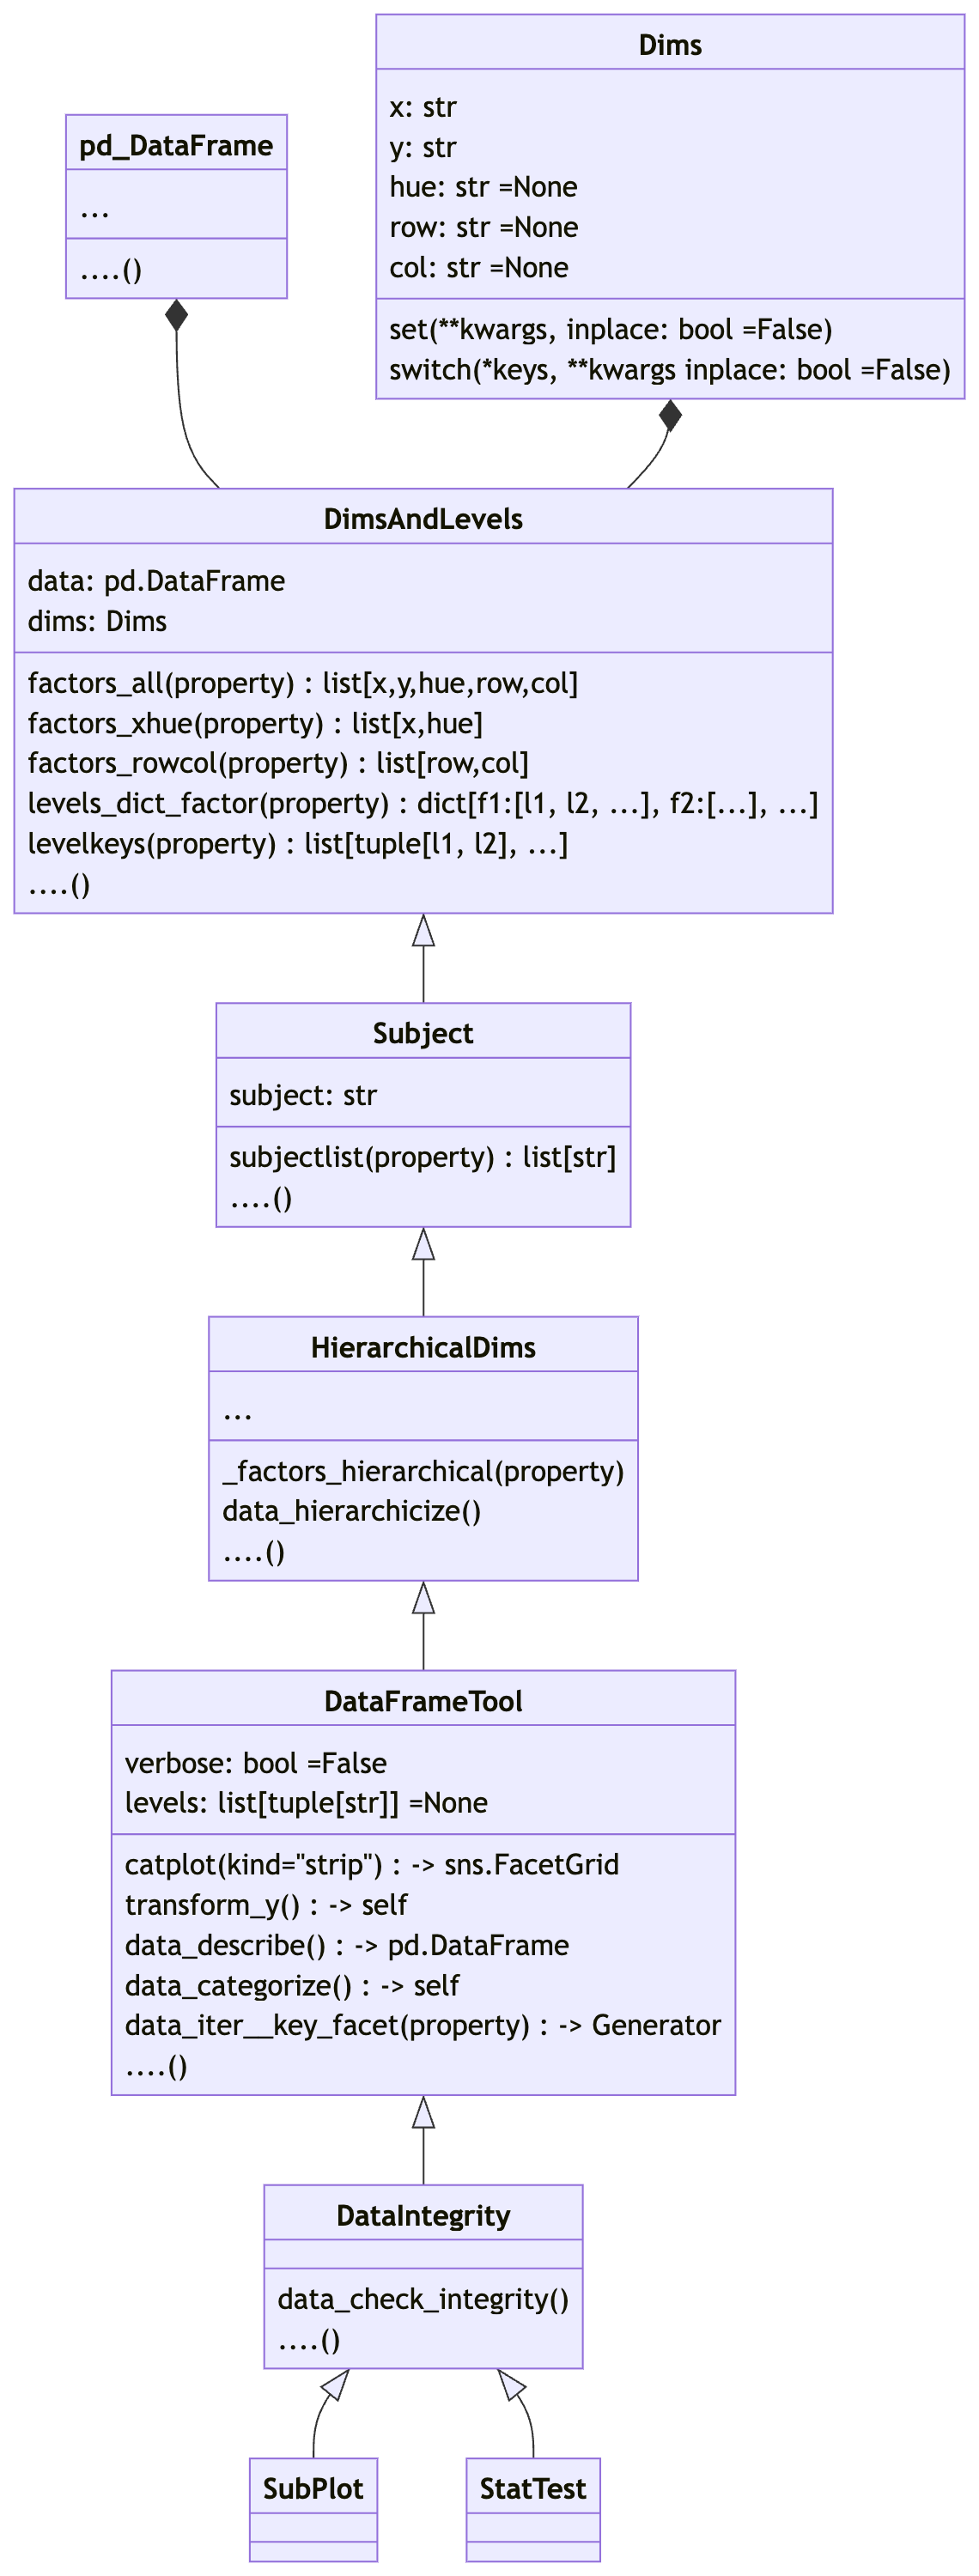
\includegraphics[scale=.18]{APPENDIX_A/classdiagr_dataframe.png}
    \caption{\mycap}
    \label{fig:classdiagr}
\end{figure}
\newpage

\setcounter{figure}{0} % > Reset figure counter
% > Lower part of Diagram
\def\mycap{\textbf{(continued)} The architecture of \texttt{plotastic}
    continues after the class \texttt{DataIntegrity} with classes for plotting
    (\texttt{SubPlot}) and statistical testing (\texttt{StatTest}) and end with
    the class \texttt{DataAnalysis}, which serves as the main user interface.
    \umlconvention }
\begin{figure}[H]
    \centering
    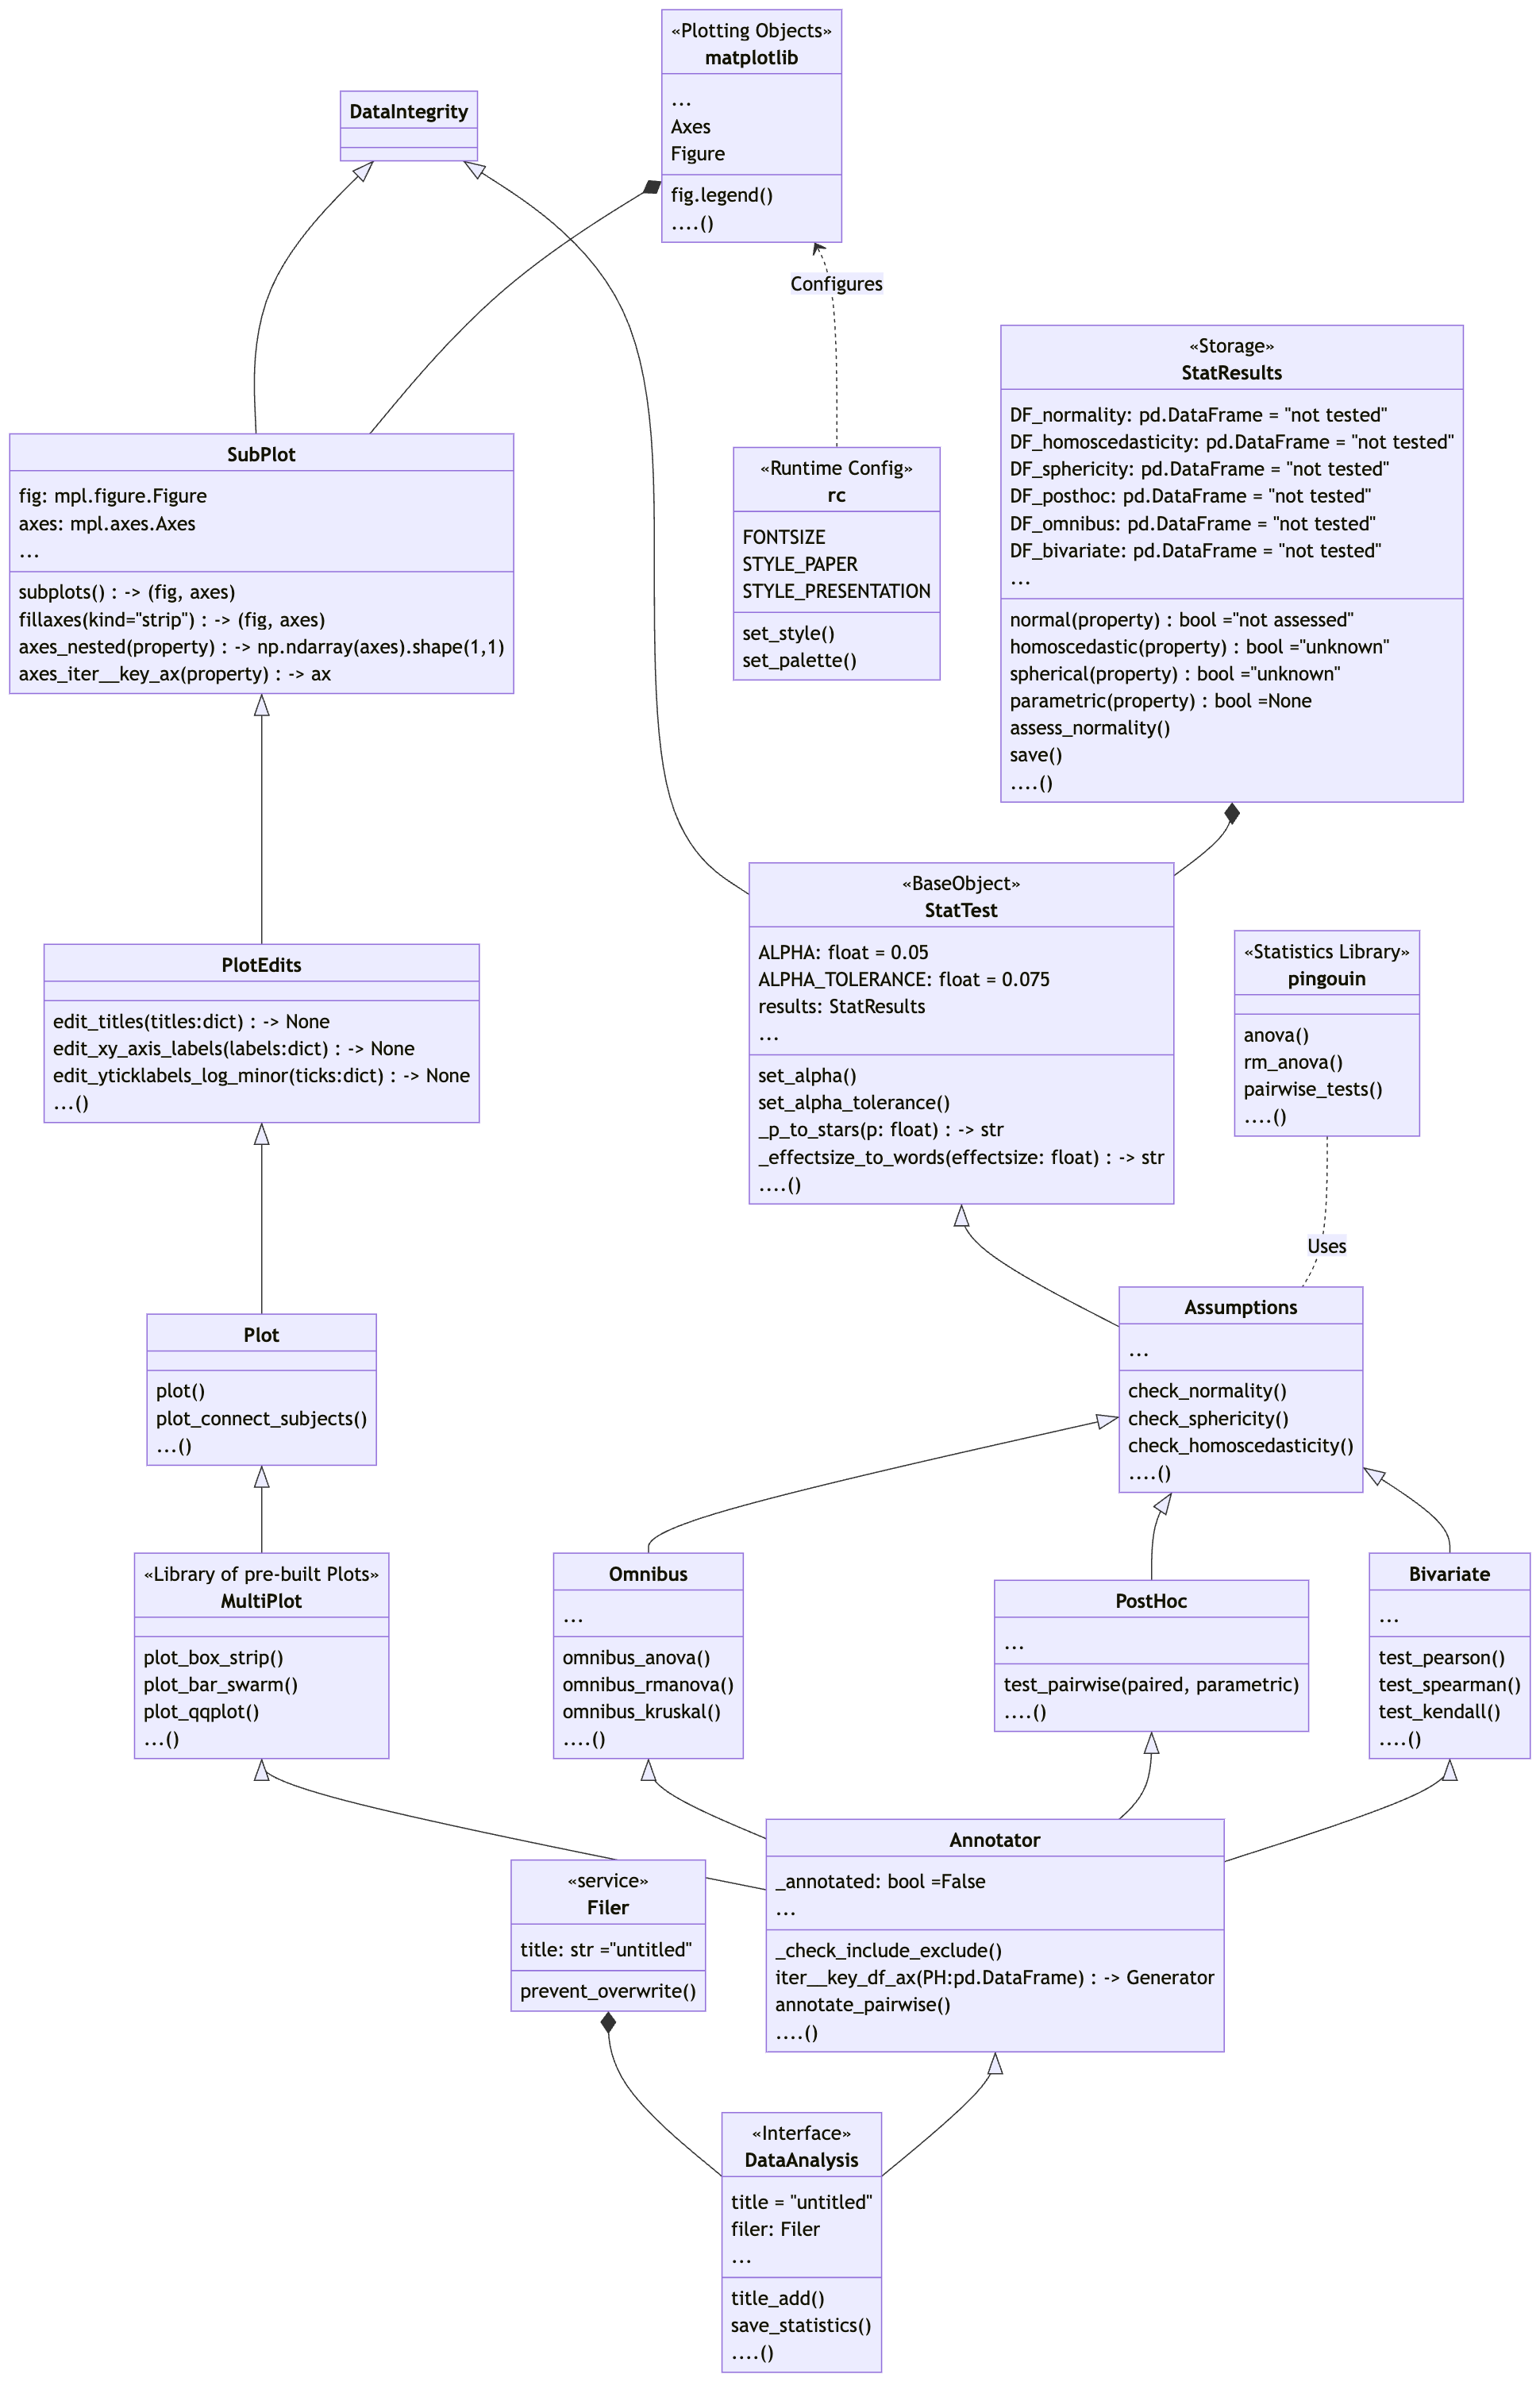
\includegraphics[scale=.20]{APPENDIX_A/classdiagr_plot+stats.png}
    \caption{\mycap}
\end{figure}


% == Readme from plotastic (PyPi) ======================================
% > Make an empty page with the section title
\def\mytitle{Readme of \texttt{plotastic}}
\markboth{Appendix}{: \mytitle}
\subsection*{\mytitle}
\label{subsec:readme}
\ %
The following pages are the \texttt{README.md} of \texttt{plotastic} found in
the Python Package Index (PyPi) (\url{pypi.org/project/plotastic}), and on
GitHub (\url{github.com/markur4/plotastic}).

\addpdf[.93]{\mytitle}{APPENDIX_A/README_pypi.pdf}
\newpage




% == Example Analyses plotastic =======================================
% > Make an empty page with the section title
\def\mytitle{Example Analysis ``qpcr'' using \texttt{plotastic}}
\markboth{Appendix}{: \mytitle}
\subsection*{\mytitle}
\label{subsec:example_analysis}
\ %
The following pages are a jupyter notebook from an example analysis using
\texttt{plotastic} that's found on GitHub (\url{github.com/markur4/plotastic}).
The Dataset is derived from Chapter 1 qPCR of this thesis, exchanging the
original gene names with random ones, while preserving gene classes. 

\addpdf[.97]{\mytitle}{APPENDIX_A/qpcr.pdf}
\newpage



% ======================================================================
% == Appendix B
% ======================================================================

% == Blank page ========================================================
% > Make a page to mark start of appendix
\def\appendixb{Appendix B} % > Define the appendix title to be reused
\markboth{\appendixb}{}
\unnsection{\appendixb}
\newpage



% == Author Contributions ==============================================
\markboth{\appendixb}{: Author Contributions}
\addpdf{Author Contributions to Research Projects}{APPENDIX_B/Statement_on_ind_author_contributions_4-2022.pdf}
\newpage

\addpdf{Author Contributions to Figures and Tables}{APPENDIX_B/Statement_of_individual_author_contributions_to_figures_tables_4-2022.pdf}
\newpage




% == Affidavit / Eidestattliche Erklärung ==============================
% \unnsection{Affidavit}
% \markboth{Affidavit}{}
\addpdf{Affidavit}{APPENDIX_B/Affidavit.pdf}
\newpage


% == CV ================================================================
\addpdf{Curriculum Vitae}{APPENDIX_B/CV Martin Kuric (eng).pdf}
\newpage
